%----------------------------------------------------------------------------------------
%	PACKAGES AND OTHER DOCUMENT CONFIGURATIONS
%----------------------------------------------------------------------------------------

\documentclass{article}

\usepackage{fancyhdr} % Required for custom headers
\usepackage{lastpage} % Required to determine the last page for the footer
\usepackage{extramarks} % Required for headers and footers
\usepackage[usenames,dvipsnames]{color} % Required for custom colors
\usepackage{pgf} % Required to insert pgf plots from matplotlib
\usepackage{graphicx} % Required to insert images
\usepackage{listings} % Required for insertion of code
\usepackage{courier} % Required for the courier font
\usepackage{lipsum} % Used for inserting dummy 'Lorem ipsum' text into the template
\usepackage[utf8]{inputenc}
\usepackage[ngerman]{babel}
\usepackage{multirow}

% Margins
\topmargin=-0.45in
\evensidemargin=0in
\oddsidemargin=0in
\textwidth=6.5in
\textheight=9.0in
\headsep=0.25in

\linespread{1.1} % Line spacing

% Set up the header and footer
\pagestyle{fancy}
%\lhead{\hmwkAuthorName} % Top left header
\chead{\hmwkClass\ : \hmwkTitle} % Top center head
\rhead{\firstxmark} % Top right header
\lfoot{\lastxmark} % Bottom left footer
\cfoot{} % Bottom center footer
\rfoot{Page\ \thepage\ of\ \protect\pageref{LastPage}} % Bottom right footer
\renewcommand\headrulewidth{0.4pt} % Size of the header rule
\renewcommand\footrulewidth{0.4pt} % Size of the footer rule

\setlength\parindent{0pt} % Removes all indentation from paragraphs

%----------------------------------------------------------------------------------------
%	CODE INCLUSION CONFIGURATION
%----------------------------------------------------------------------------------------

\definecolor{MyDarkGreen}{rgb}{0.0,0.4,0.0} % This is the color used for comments
\lstloadlanguages{Perl} % Load Perl syntax for listings, for a list of other languages supported see: ftp://ftp.tex.ac.uk/tex-archive/macros/latex/contrib/listings/listings.pdf
\lstset{language=Perl, % Use Perl in this example
        frame=single, % Single frame around code
        basicstyle=\small\ttfamily, % Use small true type font
        keywordstyle=[1]\color{Blue}\bf, % Perl functions bold and blue
        keywordstyle=[2]\color{Purple}, % Perl function arguments purple
        keywordstyle=[3]\color{Blue}\underbar, % Custom functions underlined and blue
        identifierstyle=, % Nothing special about identifiers                                         
        commentstyle=\usefont{T1}{pcr}{m}{sl}\color{MyDarkGreen}\small, % Comments small dark green courier font
        stringstyle=\color{Purple}, % Strings are purple
        showstringspaces=false, % Don't put marks in string spaces
        tabsize=5, % 5 spaces per tab
        %
        % Put standard Perl functions not included in the default language here
        morekeywords={rand},
        %
        % Put Perl function parameters here
        morekeywords=[2]{on, off, interp},
        %
        % Put user defined functions here
        morekeywords=[3]{test},
       	%
        morecomment=[l][\color{Blue}]{...}, % Line continuation (...) like blue comment
        numbers=left, % Line numbers on left
        firstnumber=1, % Line numbers start with line 1
        numberstyle=\tiny\color{Blue}, % Line numbers are blue and small
        stepnumber=5 % Line numbers go in steps of 5
}

% Creates a new command to include a perl script, the first parameter is the filename of the script (without .pl), the second parameter is the caption
\newcommand{\perlscript}[2]{
\begin{itemize}
\item[]\lstinputlisting[caption=#2,label=#1]{#1.pl}
\end{itemize}
}

%----------------------------------------------------------------------------------------
%	DOCUMENT STRUCTURE COMMANDS
%	Skip this unless you know what you're doing
%----------------------------------------------------------------------------------------

% Header and footer for when a page split occurs within a problem environment
\newcommand{\enterProblemHeader}[1]{
%\nobreak\extramarks{#1}{#1 continued on next page\ldots}\nobreak
%\nobreak\extramarks{#1 (continued)}{#1 continued on next page\ldots}\nobreak
}

% Header and footer for when a page split occurs between problem environments
\newcommand{\exitProblemHeader}[1]{
%\nobreak\extramarks{#1 (continued)}{#1 continued on next page\ldots}\nobreak
%\nobreak\extramarks{#1}{}\nobreak
}

\setcounter{secnumdepth}{0} % Removes default section numbers
\newcounter{homeworkProblemCounter} % Creates a counter to keep track of the number of problems

\newcommand{\homeworkProblemName}{}
\newenvironment{homeworkProblem}[1][Problem \arabic{homeworkProblemCounter}]{ % Makes a new environment called homeworkProblem which takes 1 argument (custom name) but the default is "Problem #"
\stepcounter{homeworkProblemCounter} % Increase counter for number of problems
\renewcommand{\homeworkProblemName}{#1} % Assign \homeworkProblemName the name of the problem
\section{\homeworkProblemName} % Make a section in the document with the custom problem count
%\enterProblemHeader{\homeworkProblemName} % Header and footer within the environment
}{
%\exitProblemHeader{\homeworkProblemName} % Header and footer after the environment
}

\newcommand{\problemAnswer}[1]{ % Defines the problem answer command with the content as the only argument
\noindent\framebox[\columnwidth][c]{\begin{minipage}{0.98\columnwidth}#1\end{minipage}} % Makes the box around the problem answer and puts the content inside
}

\newcommand{\homeworkSectionName}{}
\newenvironment{homeworkSection}[1]{ % New environment for sections within homework problems, takes 1 argument - the name of the section
\renewcommand{\homeworkSectionName}{#1} % Assign \homeworkSectionName to the name of the section from the environment argument
\subsection{\homeworkSectionName} % Make a subsection with the custom name of the subsection
%\enterProblemHeader{\homeworkProblemName\ [\homeworkSectionName]} % Header and footer within the environment
}{
%\enterProblemHeader{\homeworkProblemName} % Header and footer after the environment
}

%----------------------------------------------------------------------------------------
%	NAME AND CLASS SECTION
%----------------------------------------------------------------------------------------

\newcommand{\hmwkTitle}{Übung\ \#4} % Assignment title
\newcommand{\hmwkDueDate}{Montag,\ 17.\ November\ 2014} % Due date
\newcommand{\hmwkClass}{Introduction to HPC} % Course/class
\newcommand{\hmwkClassTime}{} % Class/lecture time
\newcommand{\hmwkClassInstructor}{} % Teacher/lecturer
\newcommand{\hmwkAuthorName}{Günther Schindler, Christoph Klein, Klaus Naumann} % Your name

%----------------------------------------------------------------------------------------
%	TITLE PAGE
%----------------------------------------------------------------------------------------

\title{
\vspace{2in}
\textmd{\textbf{\hmwkClass:\ \hmwkTitle}}\\
\normalsize\vspace{0.1in}\small{Abgabe\ am\ \hmwkDueDate}\\
\vspace{0.1in}\large{\textit{\hmwkClassTime}}
\vspace{3in}
}

\author{\textbf{\hmwkAuthorName}}
\date{} % Insert date here if you want it to appear below your name

%----------------------------------------------------------------------------------------

\begin{document}

\maketitle

%----------------------------------------------------------------------------------------
%	TABLE OF CONTENTS
%----------------------------------------------------------------------------------------

%\setcounter{tocdepth}{1} % Uncomment this line if you don't want subsections listed in the ToC

\newpage
\tableofcontents
\newpage

%----------------------------------------------------------------------------------------
%	Review
%----------------------------------------------------------------------------------------

\begin{homeworkProblem}[Review 'The future of microprocessors']
Shekhar Borkar and Andrew A. Chien analyse in 'The future of microprocessors' the
challenges for continued performance scaling caused by diminishing transistor-speed scaling
and practical energy limits. In their contribution they examine the techniques, which are
responsible for Moore's Law scaling and microprocessor performance over the past 20 years,
and show their limitations relating to the next 20 years. The contribution predicts
continuing improvement in transistor density but comparatively little improvement in transistor
speed and energy.
\\
The key insight of the contribution is, that Moore's Law continues but demands radical 
changes in architecture and software. Architectures will go beyond homogeneous parallelism,
embrace heterogeneity, and exploit the bounty of transistors to incorporate 
application-customized hardware. Software must increase parallelism and expoit heterogeneous
and apllication-customized hardware to deliver performance growth.
\\
The challenge of performance increasing will still be a important issue in the next decades,
but physical problems like transistors reache atomic dimensions will appear.
So, in my opinion the authors are right about that Moore's Law is continuing but demands on
radical changes in architecture and software. Also they are right about software and hardware
getting more application-customized, because parallelism is needed and parallelism isn't 
generic.
\end{homeworkProblem}
\clearpage
%----------------------------------------------------------------------------------------
%	Code Comments
%----------------------------------------------------------------------------------------
\begin{homeworkProblem}[Code Overview]
We solved all the tasks using one executable program. You can choose command line
options to get the different wanted outputs. A help function callable via
\texttt{-h} shows the available options. In the following you get a short overview
of the source data, which you can find in the \texttt{/src/} directory.
\begin{description}
    \item[\texttt{main.c}]\hfill\\
        Here the main work of the different processes is managed.
        Furthermore the command line options are evaluated and
        output is specified.
    \item[\texttt{distribution.c/h}] \hfill\\
        Here you can find the tree algorithm for the job distribution.
        You see a schematically description of this algorithm in figure
        \ref{fig:tree_sheme}. The algorithm always cuts the output
        matrix' area into halves until the number of working processes
        is reached.
    \item[\texttt{matrix\_multiply.c/h}] \hfill\\
        This are the functions used for exercise sheet II.
    \item[\texttt{parallel\_matmult.c/h}] \hfill\\
        This file contains the functions for communication and
        synchronization between the different processes.
        Jobs, which should be calculated, must be send to
        other processes and recieved.
    \item[\texttt{tests.c}] \hfill\\
        Here you can find test functions for the program.
\end{description}

\begin{figure}
    \begin{center}
    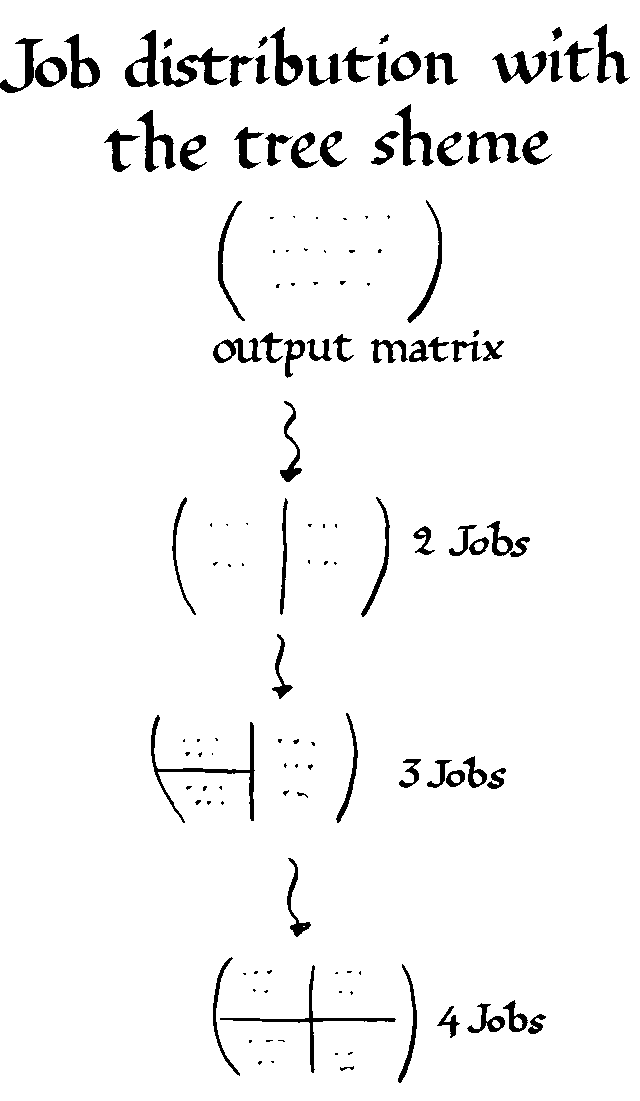
\includegraphics[width=0.6\textwidth]{./docu/tree_sheme}
    \end{center}
    \caption{the tree algorithm for job distribution. You can see
        the output matrix' area, which is divided into pieces, which
        should be calculated by one process.}
    \label{fig:tree_sheme}
\end{figure}
\end{homeworkProblem}
\clearpage
%----------------------------------------------------------------------------------------
%	Matrix multiply – parallel version using MPI
%----------------------------------------------------------------------------------------
\begin{homeworkProblem}[Matrix multiply – parallel version using MPI]

After executing the matrix multiply with 2 worker processes, we can verify the correct
behaviour of the matrix multiply as shown below.
 \begin{center}
\begin{tabular}{ |c|c|c|c|c|c| } 
\hline
C[i,j] & C[,0] & C[,1] & C[,2] & C[,3] & C[,4] \\
\hline
C[0,] & 0 & 30 & 60 & 90 & 120 \\ 
\hline
C[1,] & 0 & 40 & 80 & 120 & 160 \\ 
\hline
C[2,] & 0 & 50 & 100 & 150 & 200 \\ 
\hline
C[3,] & 0 & 60 & 120 & 180 & 240 \\
\hline
C[4,] & 0 & 70 & 140 & 210 & 280 \\
\hline
\end{tabular}
\end{center}
\end{homeworkProblem} 
\clearpage
%----------------------------------------------------------------------------------------
%	Matrix multiply – scaling process count
%----------------------------------------------------------------------------------------
\begin{homeworkProblem}[Matrix multiply – scaling process count]

\end{homeworkProblem}
\clearpage
%----------------------------------------------------------------------------------------
%	Matrix multiply – scaling problem size
%----------------------------------------------------------------------------------------
\begin{homeworkProblem}[Matrix multiply – scaling problem size]

\end{homeworkProblem}
\clearpage
\end{document}
